\documentclass[12pt]{article}

% Any percent sign marks a comment to the end of the line

% Every latex document starts with a documentclass declaration like this
% The option dvips allows for graphics, 12pt is the font size, and article
%   is the style

\usepackage[pdftex]{graphicx}
\usepackage{url}

\usepackage{soul}

\usepackage{hyperref} % Using hyperlink

\usepackage{graphicx} % Required for including images

\usepackage{setspace}
\setstretch{1}


%\usepackage{geometry}
% \geometry{
% left=7.6cm,top=0.1cm,right=1cm,bottom=0.1cm,nohead,nofoot
% }

% These are additional packages for "pdflatex", graphics, and to include
% hyperlinks inside a document.

\setlength{\oddsidemargin}{-0.25in}
\setlength{\textwidth}{7in}
\setlength{\topmargin}{-0.8in}
\setlength{\textheight}{9.2in}

% These force using more of the margins that is the default style

\begin{document}

% Everything after this becomes content
% Replace the text between curly brackets with your own

%\title{Hong Kong Labour Market Data Visualization}
%\author{Fong Chun Him (3035377115), Wu Szu Han (3035562617)}
%\date{November 17, 2020}

% You can leave out "date" and it will be added automatically for today
% You can change the "\today" date to any text you like


%\maketitle

% This command causes the title to be created in the document

\begin{center}
\Huge{Training custom image classification and object detection models}
\end{center}

\section*{\large{1 \hspace{10pt} Introduction}}
Convolutional neural networks (CNNs) have been actively researched and adopted as large computation power and large datasets are becoming available. Numerous CNN architectures and models have been developed. CNN applications such as autonomous car, medical image analysis, face recognition and scene labelling are becoming mature [1]. Papers and practical guides give out huge amount of knowledge about CNNs. Nonetheless, as there are numerous CNN models, use cases and theories, beginners often encounter a difficulty of knowing what techniques they need to understand and implement and how to kick-start their practical projects. \\
\\
The aim and contribution of this project is to provide one example of image classification and one example of object detection to demonstrate the methodology and pipeline of classifying and detecting user-defined objects using CNNs. The underlying concepts and implementation details are explained. It is hoped that readers can grasp these concepts, utilize the provided source codes to overcome any technical challenges they encounter and intelligently select the right architecture for their real-life applications. \\
\\
Live demo: \href{https://cnn-repo.s3.ap-east-1.amazonaws.com/build/index.html}{https://cnn-repo.s3.ap-east-1.amazonaws.com/build/index.html}

\begin{center}
	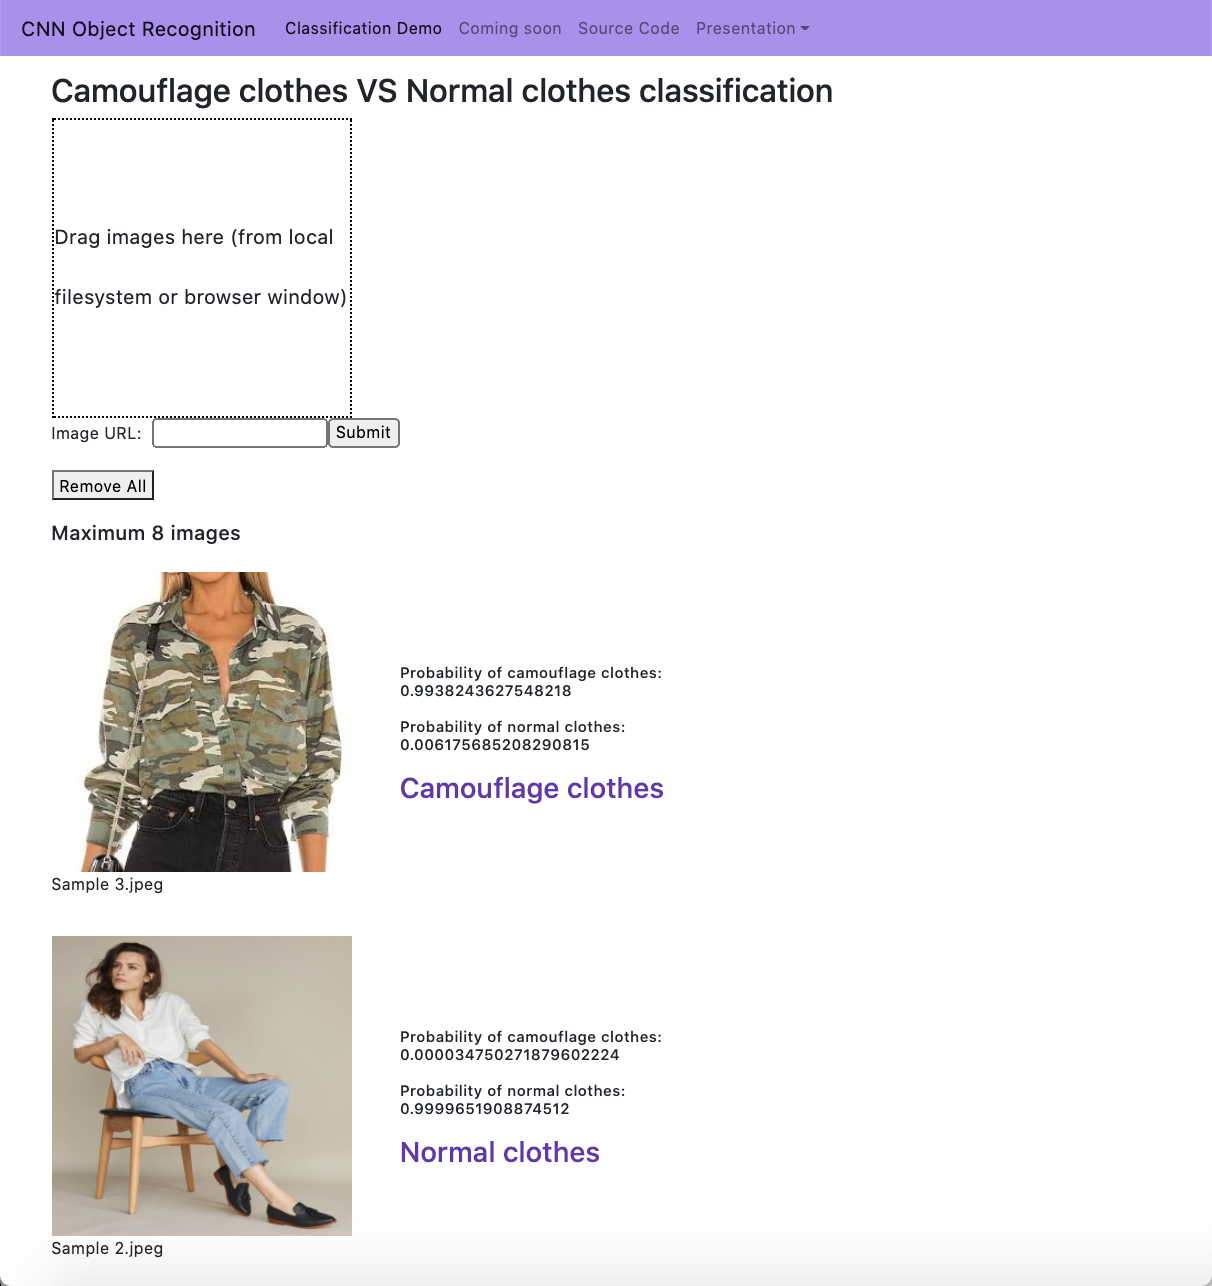
\includegraphics[width=0.6\columnwidth]{screenshot.png} % Example image
\end{center}

\section*{\large{2 \hspace{10pt} Concepts}}
Building a CNN model from scratch with random weight initialization has two major shortcomings [2]. First, large amount of data are required to collect and process to achieve high accuracy. Second, training from scratch is computationally expensive and memory-demanding. Fine-tuning, which is a type of transfer learning, can significantly reduce the number of training data and computational resources required. Data augmentation further lowers the barrier of preparing for a sufficiently large and representative dataset. Therefore, it is crucial to understand transfer learning, fine-tuning and data augmentation.

\subsection*{2.1 \hspace{10pt} Transfer Learning}
Transfer learning takes a network pre-trained on a dataset and transfers knowledge learnt from the previous training to the new task. Transfer learning is proven to help improve the accuracy and training time of CNNs [2, 3].
For startup companies and individual learners, it is too demanding to train their models from scratch. Therefore, they typically repurpose pre-trained models such as VGG19, ResNet50, Faster R-CNN and YOLO built by tech giants and star researchers to solve their specific tasks.

\subsection*{2.2 \hspace{10pt} Fine-tuning}
There are two approaches to transfer learning. They are feature extraction and fine-tuning.
Feature extraction in transfer learning is the process of using pre-trained network as a feature extractor to extract feature vectors and then feeding these feature vectors together with optional labels to a machine learning algorithm for training. Fine-tuning in transfer learning is the process of re-training the CNN in which at least some of the parameters are added or changed. It has been demonstrated that fine-tuning can boost the task accuracy when the dataset is small and different from the pre-trained model’s dataset [4]. Intuitively, since the dataset is small, it must rely on the pre-trained model to learn more basic geometric shapes. When the dataset is different from the pre-trained model's dataset, for example, knowing whether an object is a clothes is not directly helpful for differentiating clothes of different styles without adding more knowledge on top of the previous visual cognition.

\subsection*{2.3 \hspace{10pt} Data Augmentation}


\section*{\large{3 \hspace{10pt} Implementations}}
hello

\subsection*{3.1 \hspace{10pt} Image Classification}
hello

\subsection*{3.2 \hspace{10pt} Object Detection}
hello



\section*{\large{4 \hspace{10pt} Conclusion}}

\section*{\large{5 \hspace{10pt} References}}
[1] https://ijcsit.com/docs/Volume\%207/vol7issue5/ijcsit20160705014.pdf
[2] https://openreview.net/pdf?id=ryxyCeHtPB
[3] https://www.researchgate.net/profile/Jordan-Bird/publication/325803364\_A\_Study\_on\_CNN\_Transfer\_Learning\_for\_Image\_Classification/links/5bd8874b92851c6b279a23ea/A-Study-on-CNN-Transfer-Learning-for-Image-Classification.pdf
[4] https://arxiv.org/pdf/1406.2952.pdf
\end{document}